\section{实机实验}
\label{sec:experiments}
实验围绕三个问题展开：完整方法相对现有动作生成策略的表现如何，语义输入与查询监督分别带来何种收益，
以及这些收益如何随物体类别和初始位置变化。
全部结果来自完成补采后的五组实机记录，共480次有效试验。

\subsection{任务、数据与评价协议}
双臂系统执行遮挡物体操作：一侧操作遮挡布使目标暴露，另一侧使用工具将目标移出遮挡并送入指定区域，随后恢复遮挡布覆盖。
输入来自前、侧两个RGB视角，统一为$640\times360$。
示范数据包含108条轨迹、61740帧，以30 Hz记录10维关节位置和动作，训练物体为方块、纸球和螺丝。
测试增加训练未见的蜡笔，按相同任务目标评估类别变化下的表现。
这里的训练未见指动作示范中的物体类别，不涉及对视觉预训练语料的排除承诺。

每类物体设置12个位置，每位置重复两次，每种方法共96次。
位置以$(x,y)$表示，$x=0,1,2,3$从图像左向右排列，$y=0,1,2$从上向下排列。
每种方法在同一位置汇总四类物体后有8次试验；每类物体有24次。
该坐标用于描述测试网格，不赋予行号物理深度含义。

单次策略控制时限为40 s，目标控制频率为30 Hz。
统一视觉评估器使用前视角检测目标暴露、脱离遮挡、进入目标区域及遮挡布恢复，侧视角只作诊断。
完成条件要求上述状态同时成立，并在最近7次分割评估中至少获得4次成功票；
遮挡布恢复使用前视角像素占比阈值0.32。
最终统计采用保存并由操作者确认的成功或失败标签。
阶段检测是辅助证据，不以「曾到达某阶段」替代最终成功。
所有纳入记录均为正常退出且未手动中止；一次无效中止已用正常完成的补采记录替换。
附录~\ref{app:evalaudit}列出标签修正和补采处理。

\subsection{本轮测试的实现配置}
本轮最终checkpoint采用过滤后的硬标签语义图，训练读取离线标签，在线使用冻结U-Net的argmax输出和连通分量过滤。
三个任务查询分别对应可见性、工具--目标向量和目标--区域距离，每个查询包含前、侧视角独立读出头，共8个标量。
前视角工具参考点为主轴左端点，侧视角为工具质心；区域距离使用目标像素到固定区域的最大归一化距离。
辅助Smooth L1损失的尺度为0.01，分母为几何有效坐标数，质量权重直接缩放分子。
这些是本轮实验的实际配置；方法与方法附录中保留的早期表示、几何和损失形式未作为本轮实现参数使用。

\subsection{对照方法与消融设置}
ACT与Diffusion Policy（DP）为基线。
基于ACT构建四种模块配置：ACT仅使用RGB与本体信息；RGBQtoken增加关系查询监督；
segNoQtoken增加双视角语义输入；viewQtoken同时使用语义输入与关系查询，为完整方法。
图中分别简写为ACT、RGB＋Q、语义无Q和语义＋Q。
这四种配置构成语义输入与查询监督的$2\times2$对照。

四种ACT配置每次预测60步并执行30步，采用同步推理。
DP预测64步、执行30步，采用异步推理；其DDIM去噪步数在三种训练物体上为16，在蜡笔上为24。
DP比较体现相应部署配置的表现。
所有配置均关闭额外修正模块；本组结果不包含VIOLA。

主要指标为固定试验集合上的成功次数与成功率，报告总体Wilson 95\%区间作为比例不确定性的描述。
方法比较以物体--位置为区组，在每个区组内合并两方法各两次结果，以超几何分配卷积计算双侧成功次数差检验。
总体五方法的10个两两比较采用Holm校正。
试验编号不作为跨方法的一一配对依据。
检验以区组内结果可交换为零假设条件，未将采集协议表述为随机分配。

\begin{table*}[t]
\centering
\caption{五组方法的最终实机结果。单元格为成功次数/试验数（成功率，\%）；蜡笔为训练未见物体。}
\label{tab:mainresults}
\small\setlength{\tabcolsep}{5pt}
\begin{tabular}{lccccc}
\toprule
方法 & 方块 & 纸球 & 螺丝 & 蜡笔 & 总体\\
\midrule
\tableinput{results/main_table_rows.tex}
\bottomrule
\end{tabular}
\end{table*}
\begin{figure*}[t]
\centering
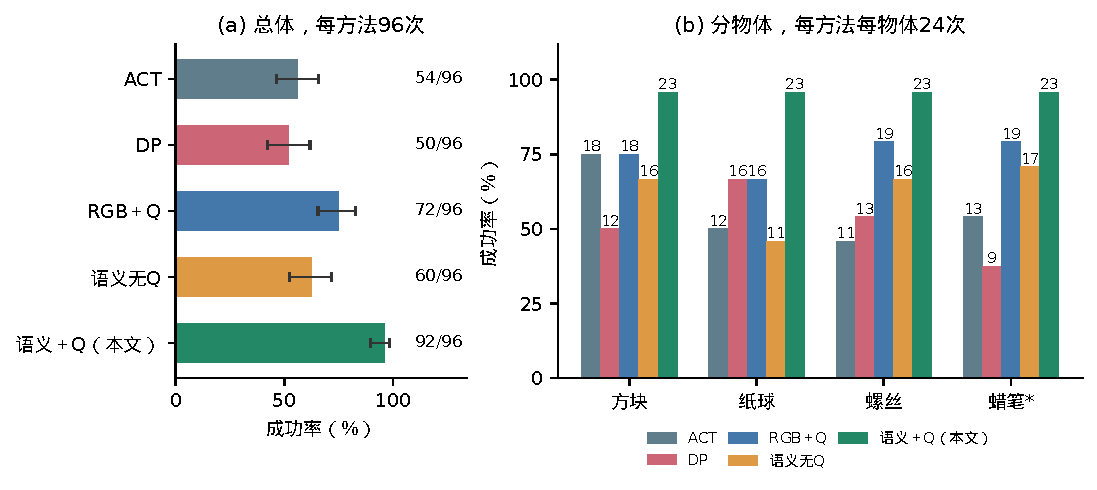
\includegraphics[width=\textwidth]{figures/results_20261023/overall_objects_zh.pdf}
\caption{总体及分物体比较。(a) 每方法96次，误差线为总体比例的Wilson 95\%区间；右侧标注成功次数。(b) 每方法每类物体24次，柱顶数字为成功次数；蜡笔标记为训练未见类别。完整方法在四类物体上均为23/24。}
\label{fig:overallobjects}
\end{figure*}

\begin{figure*}[!t]
\centering
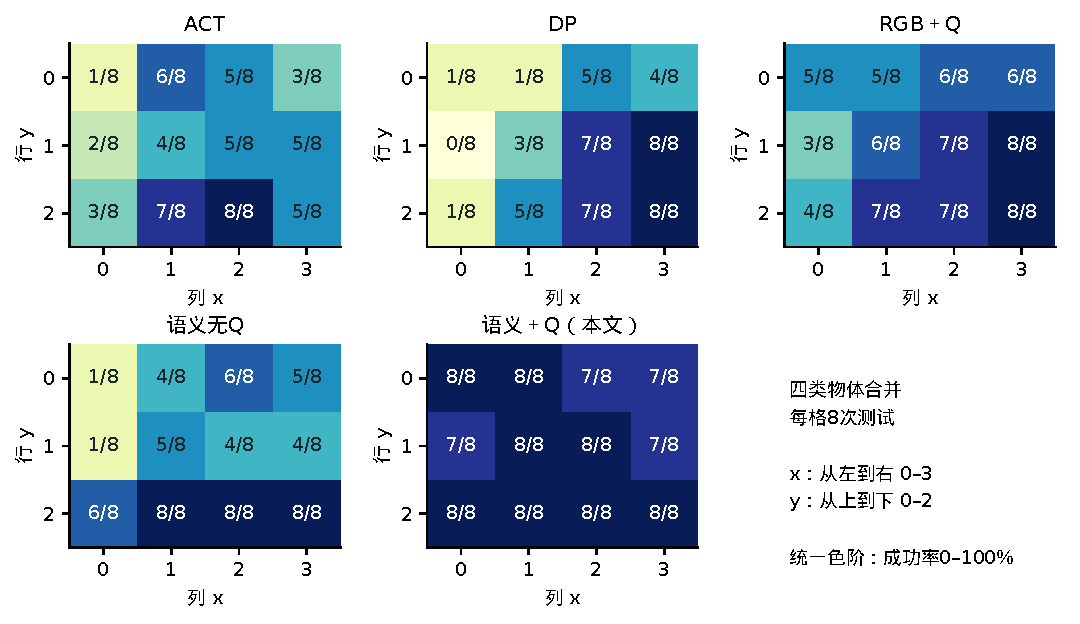
\includegraphics[width=\textwidth]{figures/results_20261023/position_zh.pdf}
\caption{相同位置下的跨物体汇总。每格为成功次数/8，统一色阶对应0--100\%成功率；横轴从左向右、纵轴从上向下。位置$(0,1)$上，ACT、DP、RGBQtoken和segNoQtoken分别为2/8、0/8、3/8和1/8，完整方法为7/8。}
\label{fig:positions}
\end{figure*}

\subsection{总体表现与物体类别}
表~\ref{tab:mainresults}和图~\ref{fig:overallobjects}显示，完整方法成功92/96次，达到95.83\%。
ACT、DP、RGBQtoken及segNoQtoken分别为54/96、50/96、72/96和60/96。
完整方法相对四组对照分别提高39.58、43.75、20.83和33.33个百分点。
总体区组检验经Holm校正后，完整方法与四组对照的差异均达到0.05水平（表~\ref{tab:contrasts}）。
RGBQtoken相对ACT和DP的校正后$p$值分别为0.0188与0.000845；
segNoQtoken相对ACT的差异未达到该水平，校正后$p=0.817$。

\begin{table}[t]
\centering
\caption{完整方法相对各对照的总体差异。成功率差以百分点计；$p$值在全部10个总体比较内校正。}
\label{tab:contrasts}
\small
\begin{tabular}{lcc}
\toprule
对照 & 成功率差 & Holm校正$p$\\
\midrule
\tableinput{results/contrast_rows.tex}
\bottomrule
\end{tabular}
\end{table}

完整方法在四类物体上均为23/24，训练物体合计69/72，蜡笔23/24，二者观察成功率同为95.83\%。
ACT和DP在三种训练物体上均为41/72，在蜡笔上分别为13/24和9/24。
RGBQtoken与segNoQtoken在蜡笔上分别为19/24与17/24，完整方法进一步提高到23/24。
按相同类别比较，完整方法相对ACT的增量分别为5、11、12和10次成功，
相对segNoQtoken为7、12、7和6次，纸球上的改进最明显。
对四类物体全部40个方法比较统一校正后，完整方法相对segNoQtoken在纸球上仍有差异证据（$p=0.00376$）；
不能将总体显著性直接推广为每个类别的单独显著性。

\subsection{语义输入与查询监督的消融}
图~\ref{fig:ablation}给出四种ACT配置。
相对RGB基线，仅增加查询监督提高18.75个百分点，仅增加语义输入提高6.25个百分点。
在查询监督存在时增加语义输入，提高20.83个百分点；
在语义输入存在时增加查询监督，提高33.33个百分点。
完整方法相对两个单模块配置分别多成功20次和32次。

两条增益之差为14.58个百分点，描述了本次试验中联合配置的额外改善。
本研究未对这一交互差异实施独立推断，因此将其作为描述性结果。
实验支持联合设计优于两个单模块配置，不能仅凭该差值断言存在显著的统计交互效应。

\begin{figure}[t]
\centering
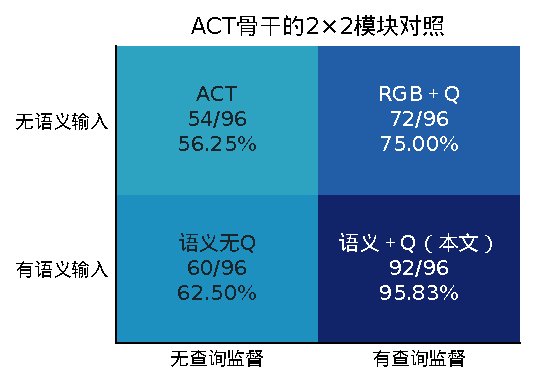
\includegraphics[width=\columnwidth]{figures/results_20261023/ablation_zh.pdf}
\caption{语义输入与查询监督的四格对照，每格96次。所有配置保留RGB和本体观测，语义输入为额外视觉流。}
\label{fig:ablation}
\end{figure}

\begin{table*}[!t]
\centering
\caption{总体比例区间与控制时长。时间不含标签保存及视频编码；成功子集平均值与全部试验平均值分别统计。}
\label{tab:timing}
\small
\begin{tabular}{lcccc}
\toprule
方法 & 成功率95\%区间（\%） & 成功子集均时（s） & 全部试验均时（s） & 20 s内成功\\
\midrule
\tableinput{results/timing_rows.tex}
\bottomrule
\end{tabular}
\end{table*}
\begin{figure*}[!t]
\centering
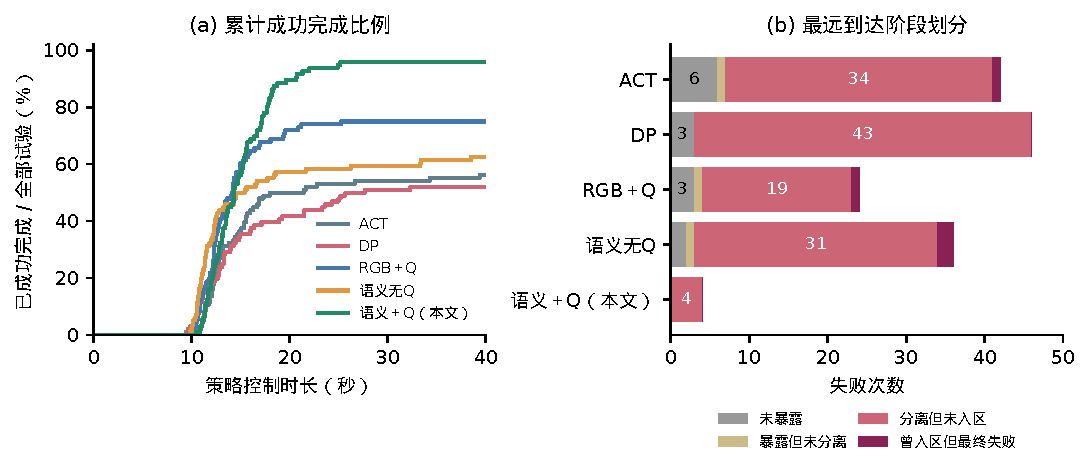
\includegraphics[width=\textwidth]{figures/results_20261023/time_failure_zh.pdf}
\caption{完成时间与失败阶段。(a) 分母固定为每方法全部96次试验，失败试验不会从分母移除。(b) 依据记录中最远到达的自动阶段与最终保存标签划分失败；边界误判经人工改为失败，保留在最后一类中。}
\label{fig:timefailure}
\end{figure*}

\subsection{位置分布与同条件重复表现}
\label{sec:positionresults}
图~\ref{fig:positions}按相同位置汇总四种物体，附录图~\ref{fig:objectpositions}进一步给出每个物体--位置的两次结果。
完整方法12个位置均至少成功7/8次；ACT范围为1/8至8/8，DP为0/8至8/8，
RGBQtoken为3/8至8/8，segNoQtoken为1/8至8/8。
因此，完整方法的观察优势体现在更多位置上保持较高成功次数。

按列汇总，每列24次，完整方法从左到右为23、24、23、22次成功，
ACT为6、17、18、13，DP为2、9、19、20，RGBQtoken为12、18、20、22，segNoQtoken为8、17、18、17。
完整方法相对RGBQtoken新增的20次成功中，17次来自左侧两列。
按行汇总，每行32次，完整方法从上到下为30、30、32，segNoQtoken为16、14、30。
二者32次成功数增量中有30次来自上方两行；segNoQtoken的36次失败中有34次位于这两行。
这些分布说明，加入查询监督后的改善并非仅来自原本容易的位置。



对位置、物体、列和行分别进行分层置换关联检验，使用200000次置换，对五方法共20项检验统一Holm校正。
DP与segNoQtoken的12位置关联分别得到$p=0.000100$和$p=0.00144$；
ACT、DP、RGBQtoken及segNoQtoken的列关联校正后$p$分别为0.0217、0.000100、0.0480和0.0258。
DP与segNoQtoken还表现出行关联，校正后$p$分别为0.0480和0.000270。
完整方法的四类关联检验均未检出差异；五种方法的物体类别关联均未达到校正后0.05水平。
未检出关联不等于证明位置或类别无影响，尤其不能仅凭不同方法各自的$p$值判定方法间的位置敏感性差异显著。

48个物体--位置条件中，两次均成功的条件数依次为ACT 17、DP 18、RGBQtoken 31、segNoQtoken 22和完整方法44。
完整方法无两次均失败的条件，其余4个条件均为一成一败，分别是方块$(3,1)$、纸球$(3,0)$、螺丝$(2,0)$和蜡笔$(0,1)$。
在相同条件的成功次数比较中，完整方法相对segNoQtoken在24个条件较好、23个相同、1个较差；
相对RGBQtoken为16个较好、30个相同、2个较差。
因此，整体改善并不意味着逐条件严格占优。

\subsection{完成时间与失败阶段}
表~\ref{tab:timing}及图~\ref{fig:timefailure}同时报告时间和失败分布。
完整方法20 s内成功86/96次，30 s内成功92/96次；
RGBQtoken相应为69/96与72/96，segNoQtoken为55/96与57/96。
成功试验的平均控制时长分别为完整方法14.77 s、RGBQtoken 13.55 s、segNoQtoken 13.80 s、ACT 14.96 s与DP 15.28 s。
各方法成功子集不同，完整方法并非成功子集平均耗时最短者。
将全部试验纳入后，完整方法平均控制时长为15.82 s，反映其更少进入超时失败。




按「曾暴露、曾分离、曾入区、最终保存成功」顺序，完整方法为96、96、92、92次，
segNoQtoken为94、93、62、60，RGBQtoken为93、92、73、72。
ACT和DP分别为90、89、55、54及93、93、50、50。
在segNoQtoken的36次失败中，31次到达分离阶段但未入区；完整方法的4次失败均属于这一阶段。
因此，完整方法的主要改善出现在分离后的目标入区过程，而剩余失败也集中于此。
「曾入区但最终失败」包含后续条件未满足以及人工标签修正，不能统一解释为恢复遮挡失败。

日志中完整方法的可训练参数为51592082个，相比ACT的51584906个增加7176个，约0.014\%。
冻结分割器使总参数量增加至76531328个。
完整方法加权平均动作块推理流水线耗时约79.24 ms，ACT约12.16 ms，DP约255.48 ms，
RGBQtoken约54.15 ms，segNoQtoken约71.20 ms。
这些日志值包含各自流水线开销，不能作为仅由查询头造成的延迟或统一硬件基准；
共享执行前缀和目标频率也不等于各方法实际控制节拍完全一致。

\begin{table*}[!t]
\centering
\caption{按最远到达阶段划分的失败计数。各列互斥，合计等于保存为失败的试验数。}
\label{tab:failurecounts}
\small
\begin{tabular}{lccccc}
\toprule
方法 & 未暴露 & 暴露未分离 & 分离未入区 & 曾入区但最终失败 & 总失败\\
\midrule
ACT & 6 & 1 & 34 & 1 & 42\\
DP & 3 & 0 & 43 & 0 & 46\\
RGBQtoken & 3 & 1 & 19 & 1 & 24\\
segNoQtoken & 2 & 1 & 31 & 2 & 36\\
viewQtoken & 0 & 0 & 4 & 0 & 4\\
\bottomrule
\end{tabular}
\end{table*}
